\documentclass[jou]{apa6}

\usepackage[american]{babel}

\usepackage{csquotes}
\usepackage[style=apa,sortcites=true,sorting=nyt,backend=biber]{biblatex}
\DeclareLanguageMapping{american}{american-apa}
\addbibresource{bibliography.bib}


%%%%%%%%%%%%%%%%%%%%%%%%%%%%%%%%%%%%%%%%
%% Discrete Structures
%% The start of RBS stuff
%%%%%%%%%%%%%%%%%%%%%%%%%%%%%%%%%%%%%%%%

% Working internal and external links in PDF
\usepackage{hyperref}
% Extra math symbols in LaTeX
\usepackage{amsmath}
\usepackage{gensymb}
\usepackage{amssymb}
% Enumerations with (a), (b), etc.
\usepackage{enumerate}

\let\OLDitemize\itemize
\renewcommand\itemize{\OLDitemize\addtolength{\itemsep}{-6pt}}

\usepackage{etoolbox}
\makeatletter
\preto{\@verbatim}{\topsep=3pt \partopsep=3pt }
\makeatother

% These sizes redefine APA for A4 paper size
\oddsidemargin 0.0in
\evensidemargin 0.0in
\textwidth 6.27in
\headheight 1.0in
\topmargin -24pt
\headheight 12pt
\headsep 12pt
\textheight 9.19in



\title{Sample Quiz 4}
\author{Discrete Structures, Spring 2020}
\affiliation{RBS}

\leftheader{Discrete Sample Quiz 6}

\abstract{%
}

%\keywords{}

\setlength\parindent{0pt}

\begin{document}

%\thispagestyle{empty}

\twocolumn
\section{Worksheet 6: Recurrent Sequences}

\vspace{10pt}
{\bf Question 1: Modifying Sudoku Rules; see Chapter 1.3.6 
(Rosen2019, p.36 ).}\\ 
We have a $9 \times 9$ table; each cell contains one number from 
$A_9 = \{ 1, 2,\ldots, 9 \}$. We define predicate $p(i,j,n)$ which 
is true iff the cell in row $i$ and column $j$ has the given value $n$.
All three arguments are integers from $1$ to $9$; this predicate is a function 
$$p \,:\, \left( A_9 \right) ^3 \rightarrow \{ \mathtt{true}, \mathtt{false} \}.$$

Formula to describe that every row $i$ contains every number: 
$$\bigwedge\limits_{i=1}^{9} \bigwedge\limits_{n=1}^{9} \bigvee_{j=1}^{9} p(i,j,k) = 
\forall i \in A_9,\;\bigwedge\limits_{n=1}^{9} \bigvee_{j=1}^{9} p(i,j,k).$$

This formula describes that each $3 \times 3$ block contains every number:
\begin{equation} 
\label{sudoku}
\bigwedge\limits_{r = 0}^{2} \bigwedge\limits_{s = 0}^{2} \bigwedge\limits_{n = 1}^{9}
\bigvee\limits_{i = 1}^{3} \bigvee\limits_{j = 1}^{3} p(3r+i, 3s+j, n).
\end{equation}

\begin{enumerate}[(A)]
\item Count the number of conjunctions ($\wedge$), disjunctions ($\vee$) and 
predicates ($p(\ldots)$) in the formula (\ref{sudoku}).
\item Similarly to the formula (\ref{sudoku}), write a Boolean formula 
to describe the following ``rule'' for sudoku tables: 
If there are any cells in the sudoku cells that have their row number difference AND column 
number difference divisible by $3$, then they contain different numbers.
For example, in Figure~\ref{fig:sudoku}, all the shaded cells have same relative position within their
respective $3 \times 3$ blocks \textendash{} therefore their row/column numbers differ by 
$0,3,6$, and accordingly to our new ``rule'' they should contain all nine different numbers. 
\end{enumerate}


\begin{figure}[!htb]
\center{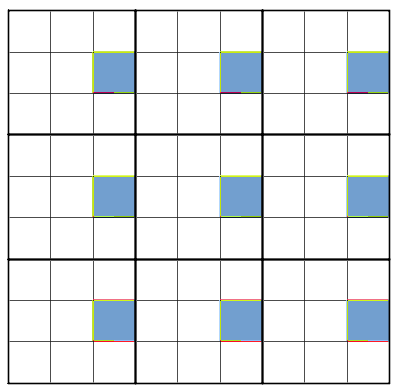
\includegraphics[width=1.4in]{quiz-sample-06/sudoku.png}}
\caption{\label{fig:sudoku} Sudoku board.}
\end{figure}




\vspace{6pt}
{\bf Question 2: Long set operations.} Denote $A_1 = \{ 1 \}$, $A_2 = \{ 1,2 \}$, etc. 
In general, $A_k = \{ 1,2,\ldots,k\}$.\\ 
By $A \oplus B = (A - B) \cup (B-A)$
we denote the symmetric difference: All elements that belong to just one of the
sets $A,B$ (but not the other one). 
Consider this set:
$$S = \bigoplus\limits_{j=1}^{100} A_j = A_1 \oplus A_2 \oplus \ldots \oplus A_{100}.$$
Write a comma-separated list of the $10$ smallest elements of $S$ in 
increasing order.

\vspace{6pt}
{\bf Question 3: Using recurrent formula.}
Find the first $5$ members of this sequence: 
$$\left\{ \begin{array}{l} 
f(0) = 1,\\
f(1) = 4,\\
f(n) = f(n - 1) \cdot f(n - 2) + 1,\; \forall n \geq 2.
\end{array} \right.$$

Write comma-separated values $f(0),f(1),f(2),f(3),f(4)$.

\vspace{6pt}
{\bf Question 4: Reccurent sequence.} A sequence of real numbers 
$f\,:\,\mathbb{N} \rightarrow \mathbb{R}$ satisfies 
the following properties:\\
{\bf (A)} $f(k+2) = f(k) + f(k+1)$ for all integers $k \geq 2$.\\
{\bf (B)} $f(n)$ is a growing geometric progression: Namely $f(1) = f(0) \cdot q$, 
$f(2) = f(0) \cdot q^2$ and so on.


Find the quotient of this geometric progression. Round it to 
the nearest thousandth (i.e. specify the first three digits after the decimal point). 

\vspace{6pt}
{\bf Question 5: Finding a limit.} Define the following sequence: 
$$\left\{ \begin{array}{l} 
x_0 = 1,\\
x_{n+1} = \frac{1}{2} \left( x_n + \frac{2}{x_n}\right),\;\text{if}\;n\geq 0\\
\end{array} \right.$$
Assume that there exists limit $L = \lim_{n \rightarrow \infty} x_n$.\\
Find that limit $L$ and round it to 
the nearest thousandth. 

\vspace{6pt}
{\bf Question 6: Find recurrent formulas.} 
We define three sequences $(a_n)_{n \in \mathbb{N}}$, 
$(b_n)_{n \in \mathbb{N}}$, $(c_n)_{n \in \mathbb{N}}$ explicitly. 
Find their recurrent formulas that allow to find next members of the 
sequence in terms of the previous ones.
\begin{itemize}
\item ${\displaystyle a_n = 2^{\frac{1}{2^n}}}$, where $n \geq 0$. 
\item $b_0 = 1$, $b_1 = 111$, $b_2 = 11111$, $b_3 = 1111111$, etc. 
(In general, the $k$th member $b_k$ has $2k+1$ digits ``1'' in its decimal notation). 
\item $c_n = n^2 + n$, where $n \geq 0$. 
\end{itemize}

\begin{tabular}{|l|l|} \hline
{\bf Initial member} & {\bf Recurrent expression} \\ \hline
$a_0 = \ldots$ & $a_{n+1} = \ldots$ (express via $a_n$ etc.) \\ \hline
$b_0 = \ldots$ & $b_{n+1} = \ldots$ \\ \hline 
$c_0 = \ldots$ & $c_{n+1} = \ldots$ \\ \hline 
\end{tabular}

\vspace{6pt}
{\bf Question 7: Taylor series} There is a formula known from calculus (practically 
used to compute $y = \sin x$) for each $x \in \mathbb{R}$. 
$$\sin x = \sum\limits_{n=0}^{\infty} \frac{(-1)^n \cdot x^{2n+1}}{(2n+1)!} = x - \frac{x^3}{3!}
+ \frac{x^5}{5!} - \ldots$$

Use Python or Scala to add the first $20$ terms of this infinite sum
to compute $\sin 30^{\circ}$. Round the answer
to the nearest thousandth.
(Taylor series expects to have argument $x$ in radians, so you have to convert degrees to radians 
before using the formula.)





\newpage

\subsection{Answers}

\vspace{6pt}
{\bf Question 1.} Answers:\\ 
{\bf (A1)} $80 = 3 \cdot 3 \cdot 9 - 1$ conjunctions.\\
{\bf (A2)} $648 = 81 \cdot 8$ disjunctions,\\
{\bf (A3)} $3 \cdot 3 \cdot 9 \cdot 3 \cdot 3 = 729$ instances of predicate $p$.\\
{\bf (B)} $\bigwedge\limits_{i = 1}^{3} \bigwedge\limits_{j = 1}^{3} \bigwedge\limits_{n = 1}^{9}
\bigvee\limits_{r = 0}^{2} \bigvee\limits_{s = 0}^{2} p(3r+i, 3s+j, n).$

\vspace{6pt}
{\bf (A1)} To count conjunctions, expand
the outer three big conjunctions in this expression:
$$\bigwedge\limits_{r = 0}^{2} \bigwedge\limits_{s = 0}^{2} \bigwedge\limits_{n = 1}^{9}
\bigvee\limits_{i = 1}^{3} \bigvee\limits_{j = 1}^{3} p(3r+i, 3s+j, n).$$
At the first step we expand the outermost $\bigwedge\limits_{r=0}^2$ 
would get three similar subexpressions:
$$\left( \mbox{let $r=0$ in}\; 
\bigwedge\limits_{s = 0}^{2} \bigwedge\limits_{n = 1}^{9}
\bigvee\limits_{i = 1}^{3} \bigvee\limits_{j = 1}^{3} p(3r+i, 3s+j, n) \right) \bigwedge$$
$$\left( \vphantom{\bigwedge\limits_{s = 0}^{2}} \mbox{let $r=1$ in}\; \ldots \right) \bigwedge 
\left( \vphantom{\bigwedge\limits_{s = 0}^{2}} \mbox{let $r=2$ in}\; \ldots \right).$$
Then we expand the next large conjunction for $s=0,1,2$. We would get $3$ smaller terms
inside every big parentheses:
{\small
$$\Big( (\ldots) \wedge (\ldots) \wedge (\ldots) \Big) \wedge
\Big( (\ldots) \wedge (\ldots) \wedge (\ldots) \Big) \wedge
\Big( (\ldots) \wedge (\ldots) \wedge (\ldots) \Big).$$
}
So far we have $8$ conjunctions: $2$ of them are between the big parentheses, 
and $3 \cdot 2 = 6$ more conjunctions separate the smaller expressions $(\ldots)$. 
After that we are ready to expand each smaller $(\ldots)$ into a conjunction of $9$ terms
for $n=1,2,\ldots,9$. 

In all we have $3 \cdot 3 \cdot 9 = 81$ expressions to separate with conjunction 
symbols ($\wedge$); we need $81-1 = 80$ such separators. 

{\bf (A2)} The number of disjunctions can be calculated in a similar manner: we have $81$ subexpressions
$\bigvee\limits_{i = 1}^{3} \bigvee\limits_{j = 1}^{3} p(3r+i, 3s+j, n)$ for all different 
combinations of $(r,s,n)$. Each subexpression has $8$ disjunctions. 

{\bf (A3)} The number of predicate instances can be counted by multiplying the 
number of elements in all five loops: $3 \cdot 3 \cdot 9 \cdot 3 \cdot 3$. 

{\bf (B)} Let us express that all the cells in the upper right corners
of all nine $3 \times 3$ blocks contain different numbers. 
One of such cells is $(i,j) = (1,1)$ (all the others can be obtained by 
adding $3$ or $6$ to $i$ and/or $j$ - thus we get nine values
$(1,1)$,$(1,4)$,$(1,7)$,
$(4,1)$,$(4,4)$,$(4,7)$,$(7,1)$,$(7,4)$,$(7,7)$). Let us express the 
statement that all the numbers $n=1,\ldots,9$ 
should appear in the shaded cells (see Figure~\ref{fig:sudoku2}):


\begin{figure}[!htb]
\center{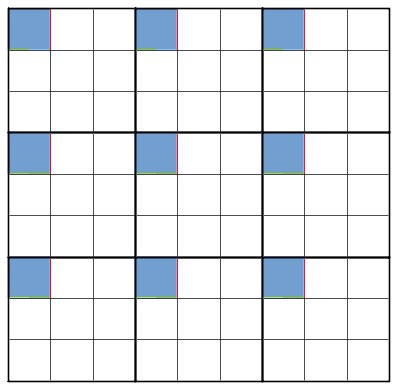
\includegraphics[width=1.4in]{quiz-sample-06/sudoku2.png}}
\caption{\label{fig:sudoku2} Sudoku board.}
\end{figure}

{\small
$$\mbox{let $i=1$,$j=1$ in}\;\forall n\in \{1,\ldots,9 \}:\;\;
\bigvee\limits_{r = 0}^{2} \bigvee\limits_{s = 0}^{2} p(3r+i, 3s+j, n).$$
}

If we want this to be true for any pair $(i,j)$, where both $i$ and $j$ take
all values $1,2,3$:
$$\bigwedge\limits_{i = 1}^{3} \bigwedge\limits_{j = 1}^{3} \bigwedge\limits_{n = 1}^{9}
\bigvee\limits_{r = 0}^{2} \bigvee\limits_{s = 0}^{2} p(3r+i, 3s+j, n).$$

\vspace{6pt}
{\bf Question 2.}\\ Answer: {\tt 2,4,6,8,10,12,14,16,18,20}\\

\begin{figure}[!htb]
\center{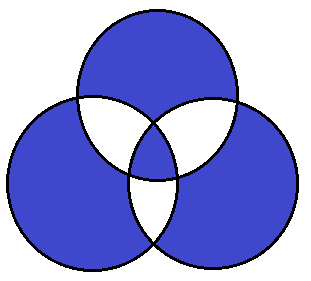
\includegraphics[width=1.4in]{quiz-sample-06/symmetric-differences.png}}
\caption{\label{fig:symmetric-differences} Symmetric differences, 3 sets.}
\end{figure}

Notice that any symmetric difference of two or more sets (Figure~\ref{fig:symmetric-differences})
includes only those elements that belong to an odd number of sets. 
For example, $A_1 \oplus A_2 \oplus A_3$ consists of the elements
that belong to exactly one set ($A_1$, $A_2$ or $A_3$), or 
all three sets: $A_1 \cap A_2 \cap A_3$. 
If you do not believe this, it can be proven by induction. 

Therefore the set $S = \bigoplus\limits_{j=1}^{100} A_j$ contains just those
elements that belong to an odd number of $A_j$. Number $1$ belongs to all $100$ sets
(therefore $1 \not\in S$). But number $2$ belongs to $99$ sets $A_j$ 
(and therefore $2 \in S$). Similarly $4 \in S$, $6 \in S$, and so on. 




\vspace{6pt}
{\bf Question 3:} Answer: {\tt 1,4,5,21,106}\\
We can verify that $f(2) = f(0)\cdot f(1) + 1 = 5$ and so on.

\vspace{6pt}
{\bf Question 4:} Answer: {\tt 1.618}\\
On one hand $f(k+2) = f(k) + f(k+1)$. On the other hand, 
$f(k) = f(0)\cdot q^k$ etc. If we plug into the above formula, we should get:
\begin{equation}
\label{some}
f(0) \cdot q^{k+2} = f(0) \cdot q^k + f(0) \cdot q^{k+1}.
\end{equation}
Since $f(k)$ is strictly increasing, we must have $f(0) \neq 0$ and 
$q > 0$. Namely, the first member in the geometric progression is nonzero, 
and the quotient is positive. 

Therefore the equation (\ref{some}) can be simplified by dividing both sides
with $f(0) \cdot q^k$:
$$q^2 = 1 + q.$$
This quadratic equation has two roots: 
$$q_{1,2} = \frac{1 \pm \sqrt{5}}{2}.$$
Only one of these roots is positive. It is approximately equal to $1.618$. 

{\em Note.} This quotient $q \approx 1.618$ is called {\em golden ratio}. 
For the regular Fibonacci numbers the ratio $F_{n+1}/F_{n}$ approaches 
this number in the limit when $n \rightarrow \infty$.


\vspace{6pt}
{\bf Question 5:} Answer: {\tt 1.414}

Since we know that the sequence 
$x_{n+1} = \frac{1}{2} \left( x_n + \frac{2}{x_n}\right)$ has a limit, then 
both $x_{n+1}$ and $x_n$ go to the same limit as $n$ grows. We have this identity:
$$L = \frac{1}{2} \left (L + \frac{2}{L} \right)$$
and therefore $L^2 =2$ and $L = \pm \sqrt{2}$. Since we start with a positive member, 
all subsequent members will be positive and $L = \sqrt{2}$.

{\em Note.} This recurrence is used in practice to calculate 
square-roots. It converges very fast. Here are the first few members with $15$ decimal digits. 
After six steps we have square root with more than $15$-digit precision.
\begin{verbatim}
x(0) = 1/1 = 1.000000000000000
x(1) = 3/2 = 1.500000000000000
x(2) = 17/12 = 1.416666666666667
x(3) = 577/408 = 1.414215686274510
x(4) = 1.414213562374690
x(5) = 1.414213562373095
x(6) = 1.414213562373095
\end{verbatim}



\vspace{6pt}
{\bf Question 6:} Answers:\\
\begin{tabular}{|l|l|} \hline
{\bf Initial member} & {\bf Recurrent expression} \\ \hline
$a_0 = 2$ & $a_{n+1} = \sqrt{a_n}$ \\ \hline
$b_0 = 1$ & $b_{n+1} = 100\cdot b_n + 11$ \\ \hline 
$c_0 = 0$ & $c_{n+1} = c_n + 2\cdot(n+1)$ \\ \hline 
\end{tabular}

{\bf (A)} Notice that the power in $a_n$ decreases twice with each step. 
So it is equivalent to taking a square-root.\\
{\bf (B)} Decimal representation of $b_{n+1}$ is easy to obtain from $b_n$: 
We first shift all the digits two places to the left (multiply by $100$), then 
add $11$ to get the last two digits equal to "11".\\
{\bf (C)} Compute the first few members of the sequence $c_n$: 
$0$, $2$, $6$, $12$, $20$. Their differences make an arithmetic progression: 
$2-0 = 2$, $6-2 = 4$, $12-6=6$, etc. So it is possible to compute the next
member by adding $2(n+1)$ (the $n$th even number).



\vspace{6pt}
{\bf Question 7:}

 


\end{document}

